% Lab report template, 07/10/2016, v. 2. This template should be used in conjunction with the PDF file generated from it.

% This is the header of your report and will not feature in the report itself. It is useful to write things like the title of the document, the date and what version the document is here. The '%' symbol starts a comment line that will not appear in the final PDF.

% This document was written with TeXstudio and compiled with TeXworks, as TeXstudio cannot compile a pdf itself. Programs like TeXworks or MiKTeX can be used exclusively for writing and compiling a document, but are less user friendly than TeXstudio.

%This template is by no means a guide on how to use LaTeX to write documents, but a brief explanation of the major differences between Microsoft Word and LaTeX is given. LaTeX is an American program, and as such, some of the commands use the American way of spelling i.e. color instead of colour. 

%  USEFUL LINKS FOR LEARNING LaTeX:
%
%   http://en.wikibooks.org/wiki/LaTeX
%
%   http://www.andy-roberts.net/writing/latex/tables
%   http://www.andy-roberts.net/writing/latex/floats_figures_captions
%   http://www.andy-roberts.net/res/writing/latex/symbols.pdf
%
\documentclass[11pt]{article} %This sets the font size and the document class of your report. In this case we use 'article' as that is ideal for shorter reports. 

% LaTeX can be enhanced by the use of packages. These packages can do many things, a few of the most common and useful are used here. They are declared before the document proper, in what is known as the 'preamble'. Packages need to be installed when a .tex file compiles into a .pdf, but should do so automatically.

\usepackage[top=2.54cm, bottom=2.54cm, left=2.75cm, right=2.75cm]{geometry} %This sets the margins of the report.
\usepackage{geometry, tikz, float, pgfplots, xcolor, titlesec, amsmath, url, hanging, siunitx, graphicx, sectsty}
\usepackage{graphicx} % A package allowing insertion of images into the text.

% Choose your citations style by commenting out one of the following groups. If you decide to change style, you should also delete the .bbl file that you will find in the same folder as your .tex and .pdf files.

% IEEE style citation:
\usepackage{cite}         % A package that creates references in the IEEE style. 
\newcommand{\citet}{\cite} % Use with cite only, so that it understands the natbib-specific \citet command
\bibliographystyle{ieeetr} % IEEE referencing (use in conjunction with the cite package)

%% Author-date style citation:
%\usepackage[round]{natbib} % A package that creates references in the author-date style, with round brackets
%\renewcommand{\cite}{\citep} % For use with natbib only: comment out for the cite package.
%\bibliographystyle{plainnat} % Author-date referencing (use in conjunction with the natbib package)


\usepackage{color} % Allows the colour of the font to be changed by using the '\color' command: This is just to support the blue comments in this template...use standard (black) text in your report.

\linespread{1.2} % Sets the spacing between lines of text.
\setlength{\parindent}{0cm}  % Suppresses indentation of text at the start of a paragraph

\begin{document} % This begins the document proper and ends the pre-amble


\begin{titlepage} % Begins the titlepage of the document
\begin{center} % Starts the beginning of an environment where all text is centered.

{\Huge Properties of Gamma Radiation}\\[0.5cm] % [0.5cm] sets the distance between this line and the next.
\textit{Jack Greenberg} and \textit{Jacob Fairham}~\\[0.3cm] % The '\\' starts a new paragraph, and will only work after a paragraph has started, unless we use '~'.
\textit{11017146} and \textit{11074241}~\\[0.3cm]
School of Physics and Astronomy~\\[0.3cm]
University of Manchester~\\[0.3cm]
Second year laboratory report~\\[0.3cm]
November 2023~\\[2cm]


\end{center}
{\Large \textbf{Abstract}}~\\[0.3cm]
 This expirement aimed to analyze the spectra created using gamma ray spectroscopy using thallium-activated sodium iodide scintillation detectors with radioactive isotopes such as $^{22}$Na, $^{60}$Co, and $^{137}$Cs. The peaks of the $^{22}$Na spectrum were then used to calculate the strength of the sodium source and the relative efficiencies of the detector at the different photopeak energies. Finally, different materials were used between the isotopes and the detector to measure the relation between gamma ray detections and the thickness of the barrier between the source and the detector at different energy levels. We found our isotope of $^{22}$Na had a source strength of $11.77\pm1.81$kBq, as compared to its theoretical $15.09$kBq obtained using the initial source strength as well as the half life of the isotope and the amount of time that has passed from the initial source measurement. We also find that, of the materials aluminium, lead, and iron, lead absorbs the most gamma rays per unit thickness and aluminium absorbs the least.

\end{titlepage}
\pagenumbering{gobble} % This stops the title page being numbered
\clearpage
\pagenumbering{arabic} % sets the style of page numbering for the report
\setcounter{page}{2} % Starts the numbering at page 2 as typically the first page is not numbered

\newpage % Starts a new page to begin the report on.

\section{Introduction} 
\label{intro}
    Gamma radiation was first discovered and studied in 1900 by Paul Villard \cite{GammaRadiation} however the first quantitative experiment was carried out by Rurtherford and Andrade in 1914; This was carried out through gamma-ray spectroscopy with a rock salt crystal and proved their wavelengths were shorter than the previously studied X-ray radiation \cite{GammaRadiation2}. In 1944, gamma-ray spectroscopy began in earnest with Curran and Baker’s development of the scintillation detector \cite{SD} which, to this day, is still the most popular method for detection of gamma rays. This experiment uses the same detection equipment to explore the three ways gamma radiation interacts with matter: Einstein’s photoelectric effect, Compton scattering and pair production. Each of these interactions produces an electron which can then be analysed to find the original energy of the photon and then processed to create a spectrum of detected photon energies. Exploring properties of gamma radiation is important as it is a powerful tool in imagery and detection. These detection techniques have been utilised to identify the presence of different radioactive isotopes which can aid geological mapping, dating of materials and are also notably used medically with many applications including predominantly imaging of inside human bodies.

\section{Theory}
    \subsection{Decay Spectra}
        The spectra obtained from measuring each source in the open air display four regions of importance. The tall, wide 'photopeaks' correspond to electrons detected through the photoelectric effect, matching the decay patterns of the isotopes. The wide spread before each photopeak represents regions of Compton background radiation, where a photon has hit an electron which is then scattered with energies dependant on the angle of scattering $\theta$. The energy of the electron following compton scattering is given by
        \begin{equation}\label{compton}
            E_{electron} = E_{initial}-\frac{E_{initial}}{1+(\frac{E_{initial}}{m_{electron}c^{2}})(1-cos\theta)}
        \end{equation}
        which comes from (citation).

        equation (1) shows that the measured energy has a maximum at $\theta$=$180^{\circ}$ which is where a drop in counts is found known as the 'Compton edge'. Inversely, at the lower energy end of compton scattering the 'backscatter peak' can be found. This is where the scattered photons return to the detector instead of the electrons and then, through the photoelectric effect, cause a low energy electron to be detected.

    \subsection{Source Strength Measurements}
        The decay process for $^{22}$Na involves two $511\unit{\keV}$ photons and one $1275\unit{\keV}$ photon. The detector comprises some fraction of the solid angle $\Omega$. The probability of a detection of a $511\unit{\keV}$ and a $1275\unit{\keV}$ photon is
        \begin{equation}
            P(511\unit{\keV}) = 2\Omega\cdot\epsilon(E=511\unit{\keV})
        \end{equation}
        \begin{equation}
            P(1275\unit{\keV}) = \Omega\cdot\epsilon(E=1275\unit{\keV})
        \end{equation}
        and the probability of the sum peak is the combination of the two probabilities.
        
        The rate of detecton for each of the peaks ($R_E$) is a measurable value and is related to the probability of the peak by
        \begin{equation}
            R_E = S\cdot P(E)
        \end{equation}
        equation (4) along with equations (2) and (3) allows the calculation of the ratio of the efficiencies of the detector at different energies
        \begin{equation}
            \frac{\epsilon(E=511\unit{\keV})}{\epsilon(E=1275\unit{\keV})} = \frac{R_{511}}{2R_{1275}}
        \end{equation}
        and the calculation of the source strength by
        \begin{equation}
            S = \frac{R_{511}\cdot R_{1275}}{R_{1786}}
        \end{equation}
    \subsection{Gamma Ray Absorption}
        It can be shown through a simple differential calculation that
        \begin{equation}
            I = I_0 e^{\frac{-x}{\tau}}
        \end{equation}
        where $\tau$ is a function of the energy/wavelength of the photon. Therefore, by categorizing the data by photopeak energy and plotting the rate of detection by the thickness of the material for each separate material, we can calculate different values of $\tau$ and relate the absorption of the materials to each other.

% \citep gives (Morin 2008), whereas \citet gives Morin (2008) which you should use if the citation is grammatically part of the sentence


% References are called to a particular place in the text by the '\cite' command. Each individual reference has an idividual label that refers to it, and it is this that is used to call it. More information on this will be given in the references section.

\section{Experimental approach}
    This experiment uses a thallium-activated sodium iodide scintillation detector to measure the spectrum of photon energies released. This consists of a rock-salt crystal connected to a photomultiplier tube (PMT) when connected to a multi-channel analyser which converts it to data the computer can process. 
    The radiation enters the NaI crystal and excites the electrons. The thallium doping of the crystal then ensures the photon released in the ensuing deexcitation is in the visible light spectrum. This is then incident with the photocathode where an electron is liberated through the photoelectric effect. The PMT then amplifies this signal by leading the electron through cups charged with a large potential difference which cause acceleration and therefore the dislodging of more electrons. By the time the signal reaches the anode at the end, the signal has been multiplied ~1,000,000x.
    This electrical signal is then sent to the multi-channel analyser which processes it into different channels corresponding to energy levels of photons. To give specific energies, data must be recorded for each source and then used with the known values of photopeak energies (citation) to calibrate each channel to an energy value.

    \begin{figure}[H] \centering \label{calibration}
        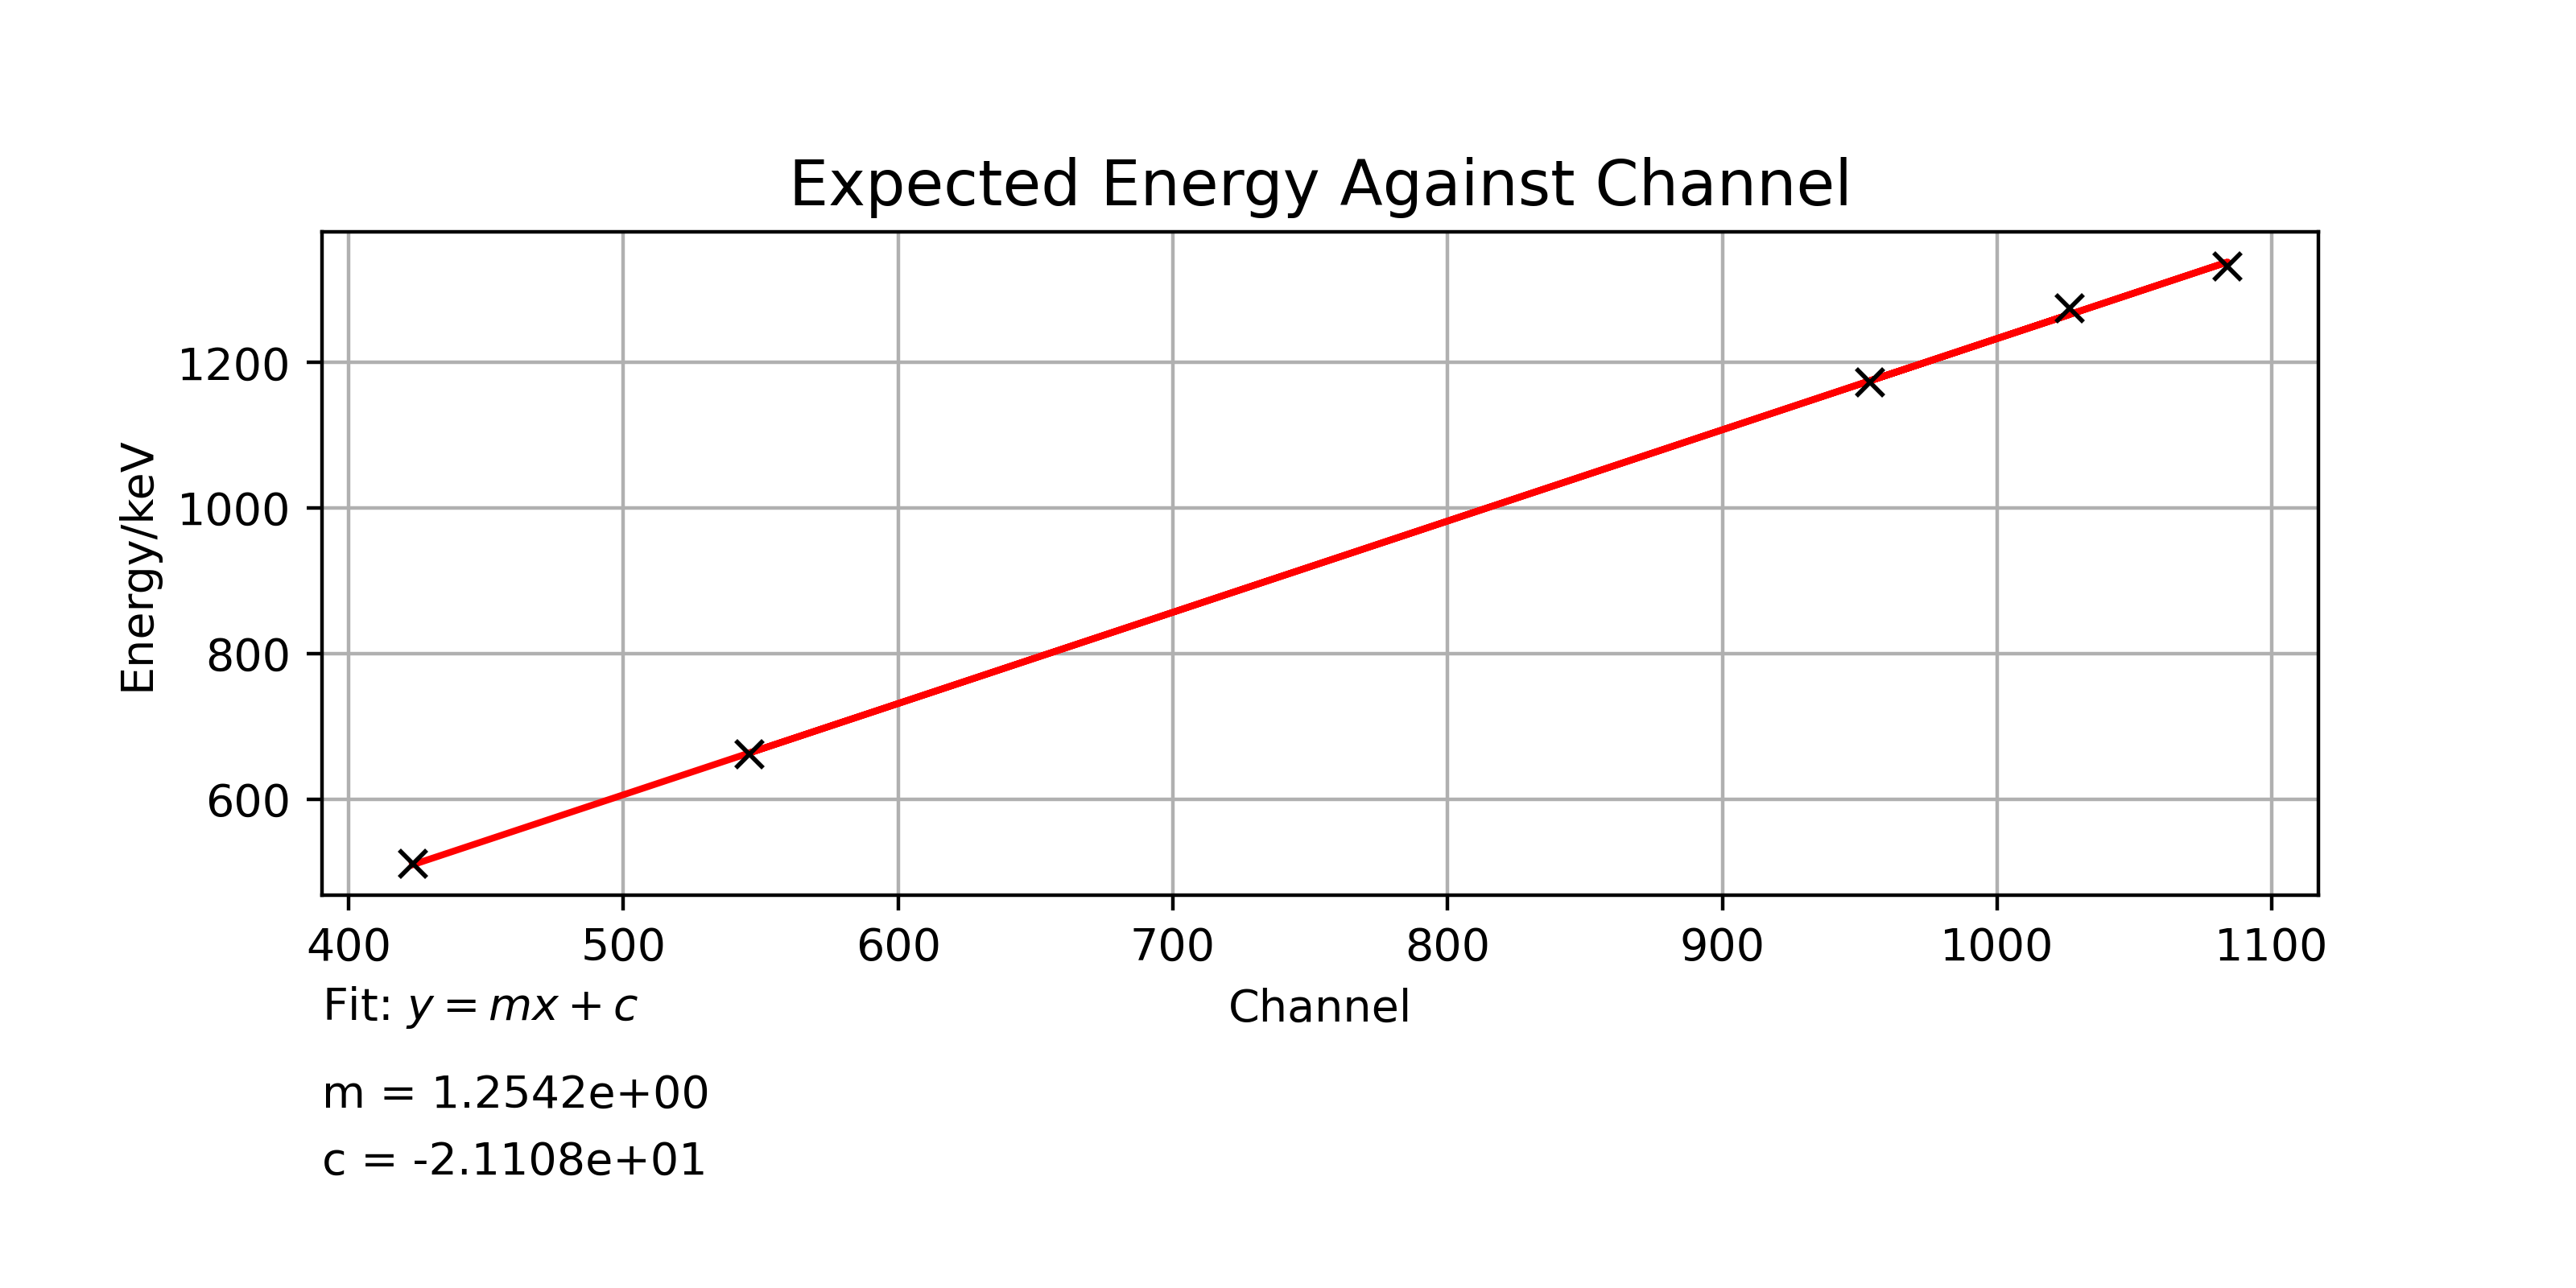
\includegraphics[scale=0.5]{assets/Calibration.png}
        \caption{LSFR plot for conversion from channels to energy}
    \end{figure}

    Figure (1) shows the relation between channel and energy to be
    \begin{equation}\label{C_to_E}
        E = 1.25C + 1.66
    \end{equation}
    where E is an energy in $\unit{\keV}$ and C is the channel number.

    the energy values obtained from running the channels through equation (2) can then be inputted to the software 'Maestro' which automatically converts all channels to their corresponding energies. In principle the channel would have some error related to the full-width half-maximum of the gaussian fit made around the peak, but such an error is not relevant to the results of this experiment. The purpose of this fit is merely to establish the relation between channels and energy values.


\section{Results}
    \subsection{Decay Spectra}
        Equation 1 predicts that we would see a compton edge and backscattering for each non-combination photopeak, which is exactly what we see.
        \begin{figure}[H] \centering \label{na22}
            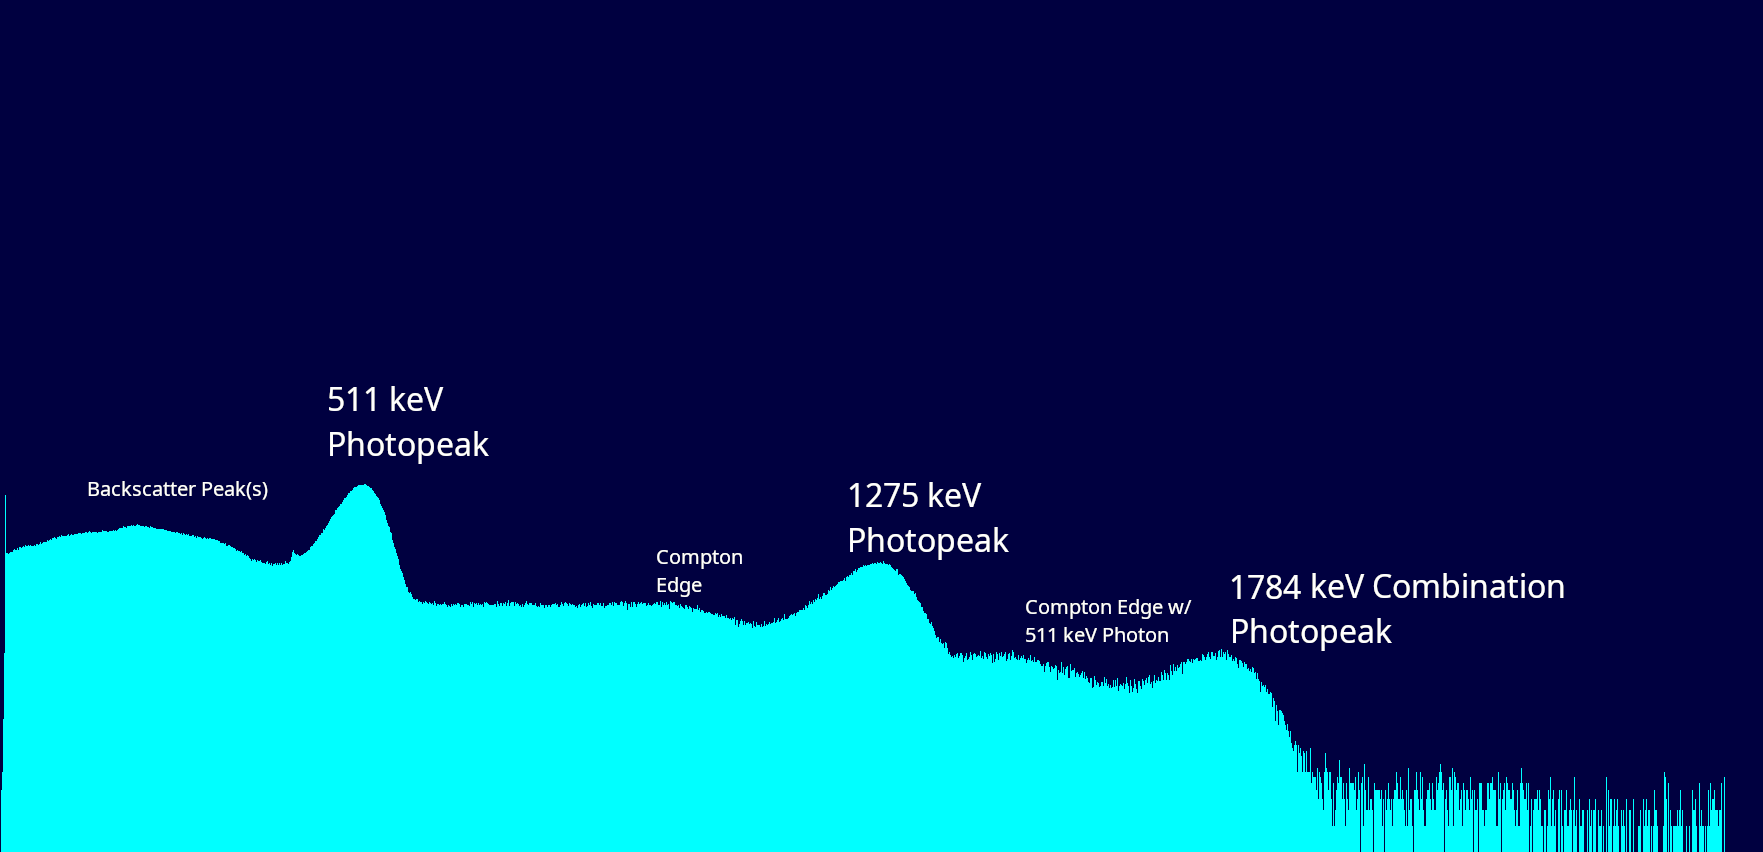
\includegraphics[scale=0.3]{assets/na22_log_annotated.png}
            \caption{Spectrum of Sodium 22 - Log scale counts by energy}
        \end{figure}
        The Sodium-22 spectrum also displays a 'sum peak' where the detector registers both the $511\unit{Kev}$ and $1275\unit{Kev}$ photons as one since the delay between the deexcitation from the 1275 line and the positron annihilation reaction is unresolvably small
        \begin{figure}[H] \centering \label{co60}
            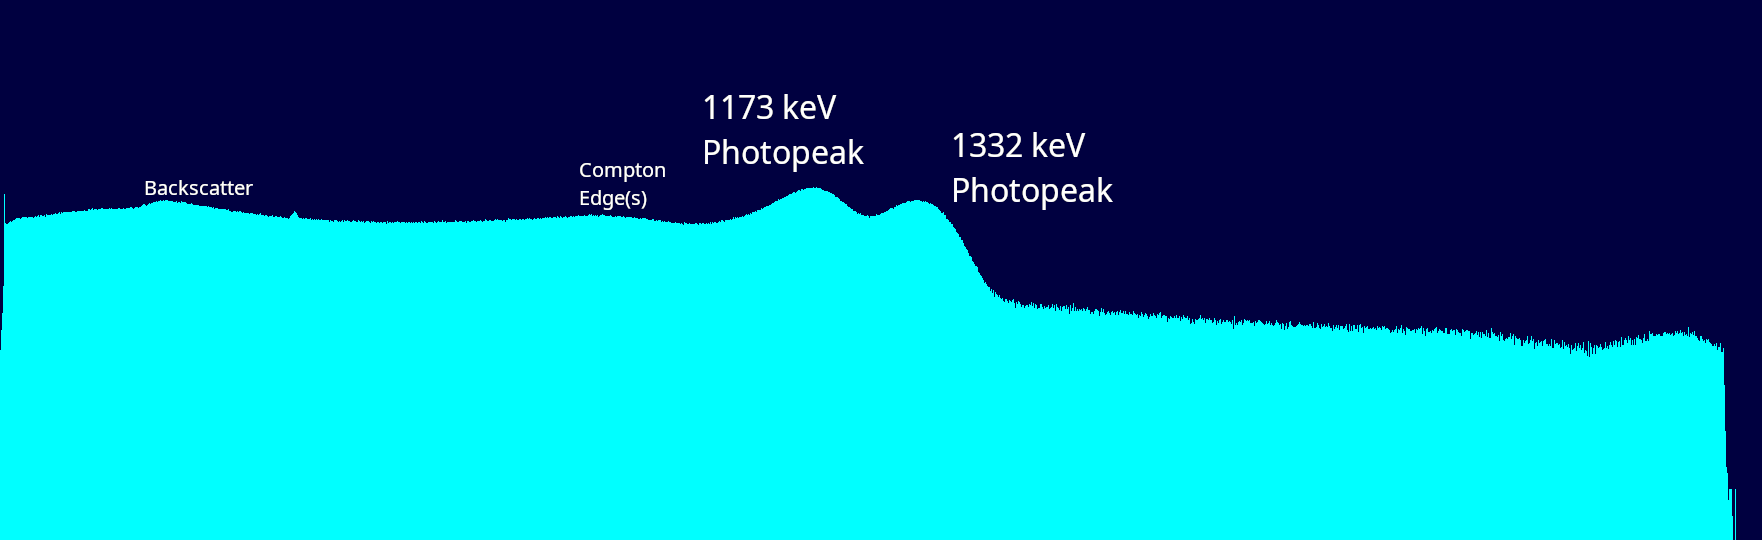
\includegraphics[scale=0.3]{assets/co60_log_annotated.png}
            \caption{Spectrum of Cobalt 60 - Log scale counts by energy}
        \end{figure}
        \begin{figure}[H] \centering \label{cs137}
            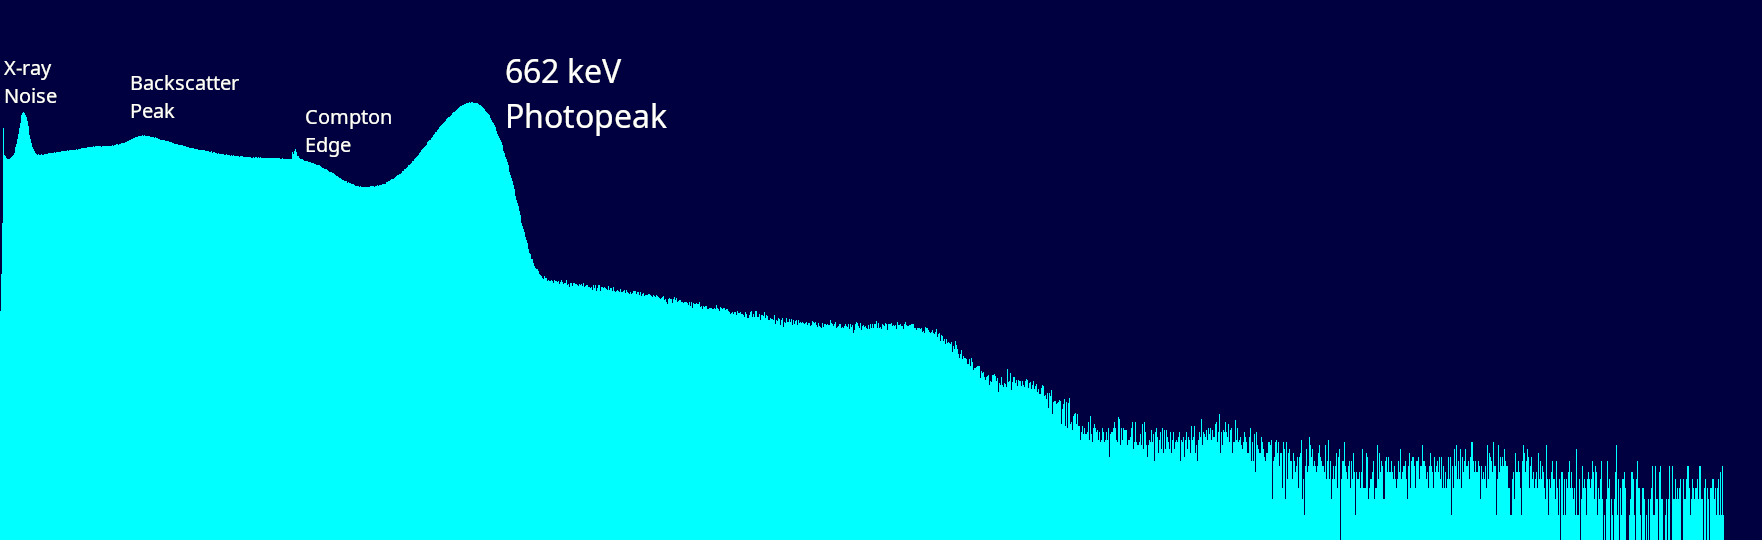
\includegraphics[scale=0.3]{assets/cs137_log_annotated.png}
            \caption{Spectrum of Cesium 137 - Log scale counts by energy}
        \end{figure}
        In figure 4, a sharp, low energy peak is seen which corresponds to X-ray radiation originating from the orbital electrons of the source as opposed to the nucleic decay producing higher energy photons.
    \subsection{Source Strength Measurements}
        Using equations (5) and (6), the source strength and efficiency ratio can be calculated from the measured data
        \begin{align*}
            R_{511} &= 202.56\pm.60\unit{\becquerel}\\
            R_{1275} &= 45.35\pm.32\unit{\becquerel}\\
            R_{1786} &= 0.78\pm.12\unit{\becquerel}
        \end{align*}
        \begin{equation}
            \frac{\epsilon(E=511\unit{\keV})}{\epsilon(E=1275\unit{\keV})} = 2.23\pm.02
        \end{equation}
        \begin{equation}
            S = 11.8\pm1.8\unit{\kilo\becquerel}
        \end{equation}
        this stands somewhat in contrast to the theoretical value calculated from an initial measurement and the half life of Sodium $22$, which evaluates to $15.09\unit{\kilo\becquerel}$. One source of error not included here is the region chosen to fit the gaussian for the sum peak, which might have caused a deviaion in the value obtained for the rate of the sum peak.
    \subsection{Gamma Ray Absorption}
        We can plot intensity as a function of the thickness of the material and we can expect the exponential curve to follow the relation described in equation 7. The following graphs represent the relation plotted for each photopeak, described by the element and the energy of the photopeak in $\unit{\keV}$ - for example, the first photopeak of Sodium 22 would be NA511. Each graph contains three curves, one for each material.
        \begin{figure}[H] \centering \label{exponentials}
            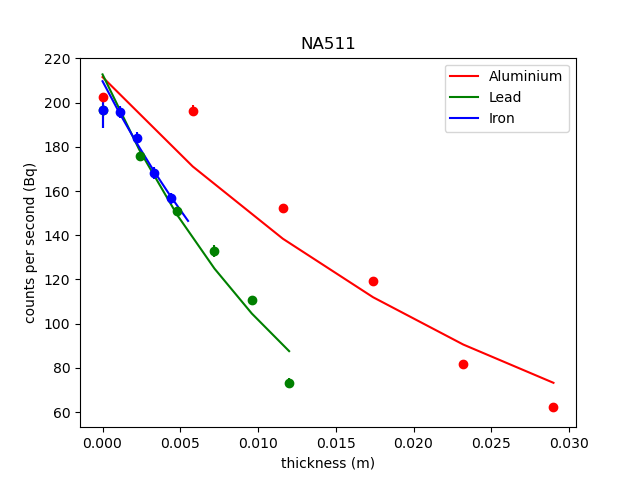
\includegraphics[scale=0.4]{assets/NA511.png}
            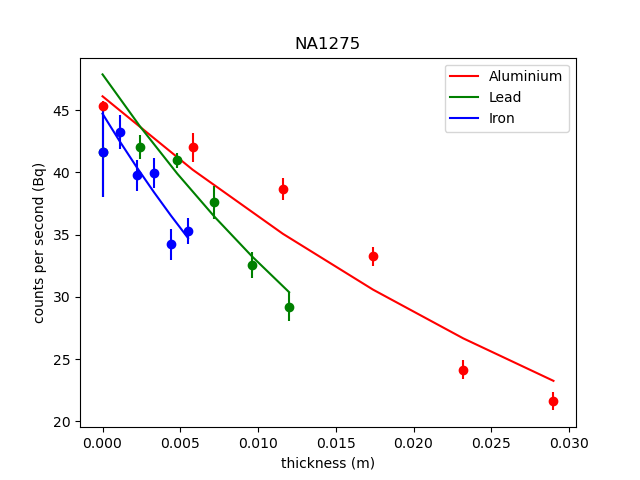
\includegraphics[scale=0.4]{assets/NA1275.png}
            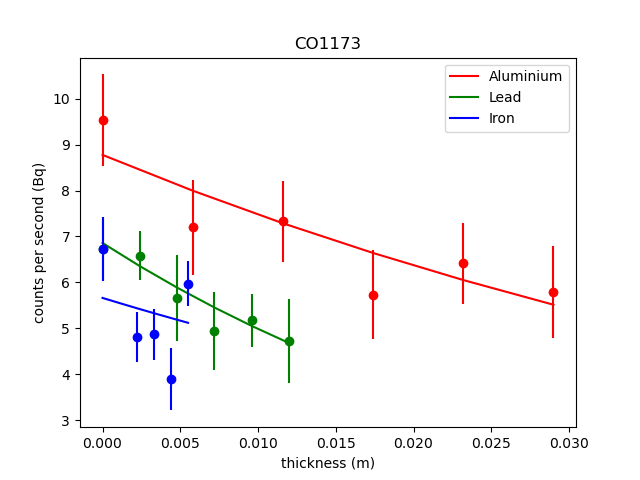
\includegraphics[scale=0.4]{assets/CO1173.png}
            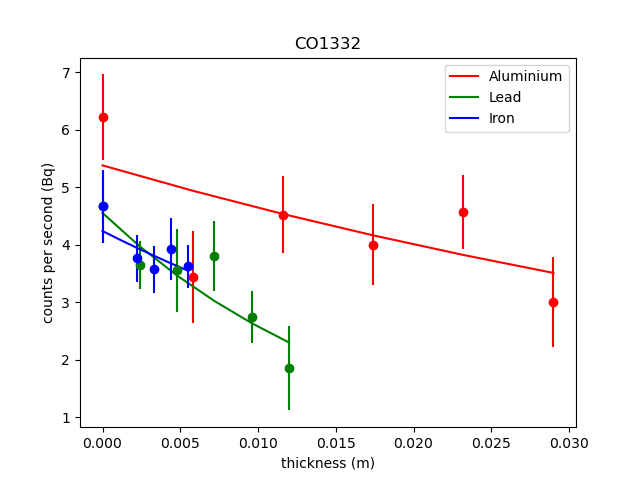
\includegraphics[scale=0.4]{assets/CO1332.png}
            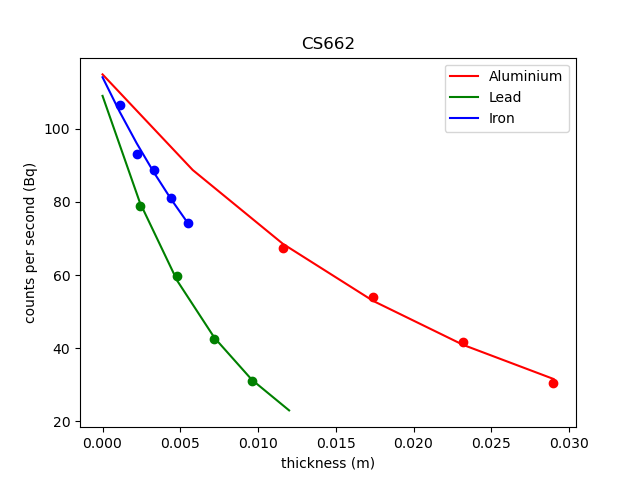
\includegraphics[scale=0.4]{assets/CS662.png}
            \caption{Counts per second measured for different thicknesses of different materials - each graph is of a different photopeak. Fit data shown below}
        \end{figure}
        \begin{table}[H] % Begins the table environment
            \begin{center}
                \begin{tabular}{ ||c|c|c|c|c|c|| }
                    $\tau$ & NA511 & NA1275 & CS662 & CO1173 & CO1332\\ 
                    Aluminium & $0.027\pm0.002$ & $0.042\pm0.005$ & $0.022\pm0.003$ & $0.062\pm0.043$ & $0.068\pm0.047$\\
                    Iron & $0.015\pm0.007$ & $0.022\pm0.015$ & $0.013\pm0.002$ & $0.055\pm0.125$ & $0.031\pm0.039$\\
                    Lead & $0.014\pm0.002$ & $0.026\pm0.009$ & $0.008\pm0.001$ & $0.031\pm0.021$ & $0.018\pm0.006$\\
                    $\chi^2$ & & & & & \\ 
                    Aluminium & $13.66$ & $4.47$ & $0.39$ & $0.59$ & $3.03$\\
                    Iron & $0.14$ & $0.49$ & $0.50$ & $4.14$ & $0.65$\\
                    Lead & $3.24$ & $0.80$ & $0.24$ & $0.23$ & $2.34$\\
                \end{tabular}
                \smallskip

                Table 1: Values of $\tau$ and $\chi^2$ for each photopeak broken down by material.
            \end{center}
        \end{table}
        It can be seen from the table that values for $\tau$ tend to be the highest for aluminium, followed by iron and then lead. Using equation (7), this implies that lead absorbs the most gamma rays per unit thickness and aluminium absorbs the least gamma rays per unit thickness with iron falling between the two. The $\chi^2$ values have an extremely large variation, which is most likely a systemic issue around having taken the data across multiple days and the exact values depending somewhat on where the boundary for the gaussian was drawn.


\section{Conclusions}
    conclusion

\bibliography{report_template_library} % Specifies the bibliography file where our references are stored. If the library file and document are not in the same folder then the file path must also be included.


\end{document}
